\chapter{Wind stress with zero buoyancy forcing}
\label{chapter:wind_alone}

In this chapter, we document a test case configured with a constant
zonal wind stress 
\begin{equation}
 \bftau  =  (0.1, 0)~\mbox{N}~\mbox{m}^{-2}
\end{equation}
and zero heat flux
\begin{equation}
Q=0~\mbox{W}~\mbox{m}^{-2}.
\end{equation}
The temperature is initialized with a stable linear stratification
according to equation (\ref{eq:linear-stratification}).  This test
ilustrates how mechanical forcing induces mixing into vertically
stratified water.  This test furthermore exercises only the local
downgradient diffusive portion of KPP, as the non-local KPP term
vanishes with a zero surface buoyancy flux.  Although somewhat
trivial, this test has proven useful for ensuring that implementation
details are consistent across ocean models making use of CVMix/KPP.

\minitoc


\section{Results from GFDL-MOM6}
\label{section:wind_only_mom6}

Figure \ref{fig:MOM6_SST_bldepth-wind_alone} shows the KPP boundary
layer depth and mixed layer depth realized from the MOM6
implementation of CVMix.  The boundary layer deepens in time, due to
the mechanical forcing from winds that eats away at the vertical
stratification.  Correspondingly, the SST cools as mixing entrains
cooler water from below.  Note how the mixed layer depth closely
follows the SST, whereas the boundary layer depth oscillates according
to the inertial oscillations.  Furthermore, note the plateaus
exhibited in the KPP boundary layer depth, particularly by the
$10~\mbox{m}$ simulation.  Such behaviour is discussed in Appendix D
of \cite{LargeKPP}.  The plateaus are less visible in the mixed layer
depth.

As furthermore discussed in Appendix D of \cite{LargeKPP}, there is a
dependence on vertical grid resolution in Figure
\ref{fig:MOM6_SST_bldepth-wind_alone}, with deeper boundary layer and
cooler SST found as the vertical grid coarsens.  The reason for the
cooler SST with coarser grids is that the KPP vertical diffusivity is
directly proportional to the boundary layer thickness, which is seen
in the lower panels of Figure \ref{fig:MOM6_SST_bldepth-wind_alone}.
Hence, deeper boundary layers produce more vertical mixing of warm
surface waters with cooler deeper waters, thus producing cooler SSTs
and warmer interior waters.  This mixing is further seen from the
depth profiles of temperature in Figure
\ref{fig:MOM6_temp-wind_alone}.  With coarser vertical grids and the
associated enhanced vertical mixing, there is an enhanced surface
cooling and deep warming relative to results from the fine vertical
grids.

Inertial oscillations in the zonal velocity are shown in Figure
\ref{fig:MOM6_zonal-wind_alone}.  The amplitude of the oscillations is
enhanced as the vertical resolution is refined.  The oscillations
impart an oscillation in the vertical shear, which in turn impacts on
the boundary layer depth.  This is the primary reason that the
boundary layer depth shows oscillations in Figure
\ref{fig:MOM6_SST_bldepth-wind_alone}.  

%%%%%%%%%%%%%%%%%%%% %%%%%%%%%%%%%%%%%%%%%%%%%
\begin{figure}[h!t]
%\rule{\textwidth}{0.005in}
\begin{center}
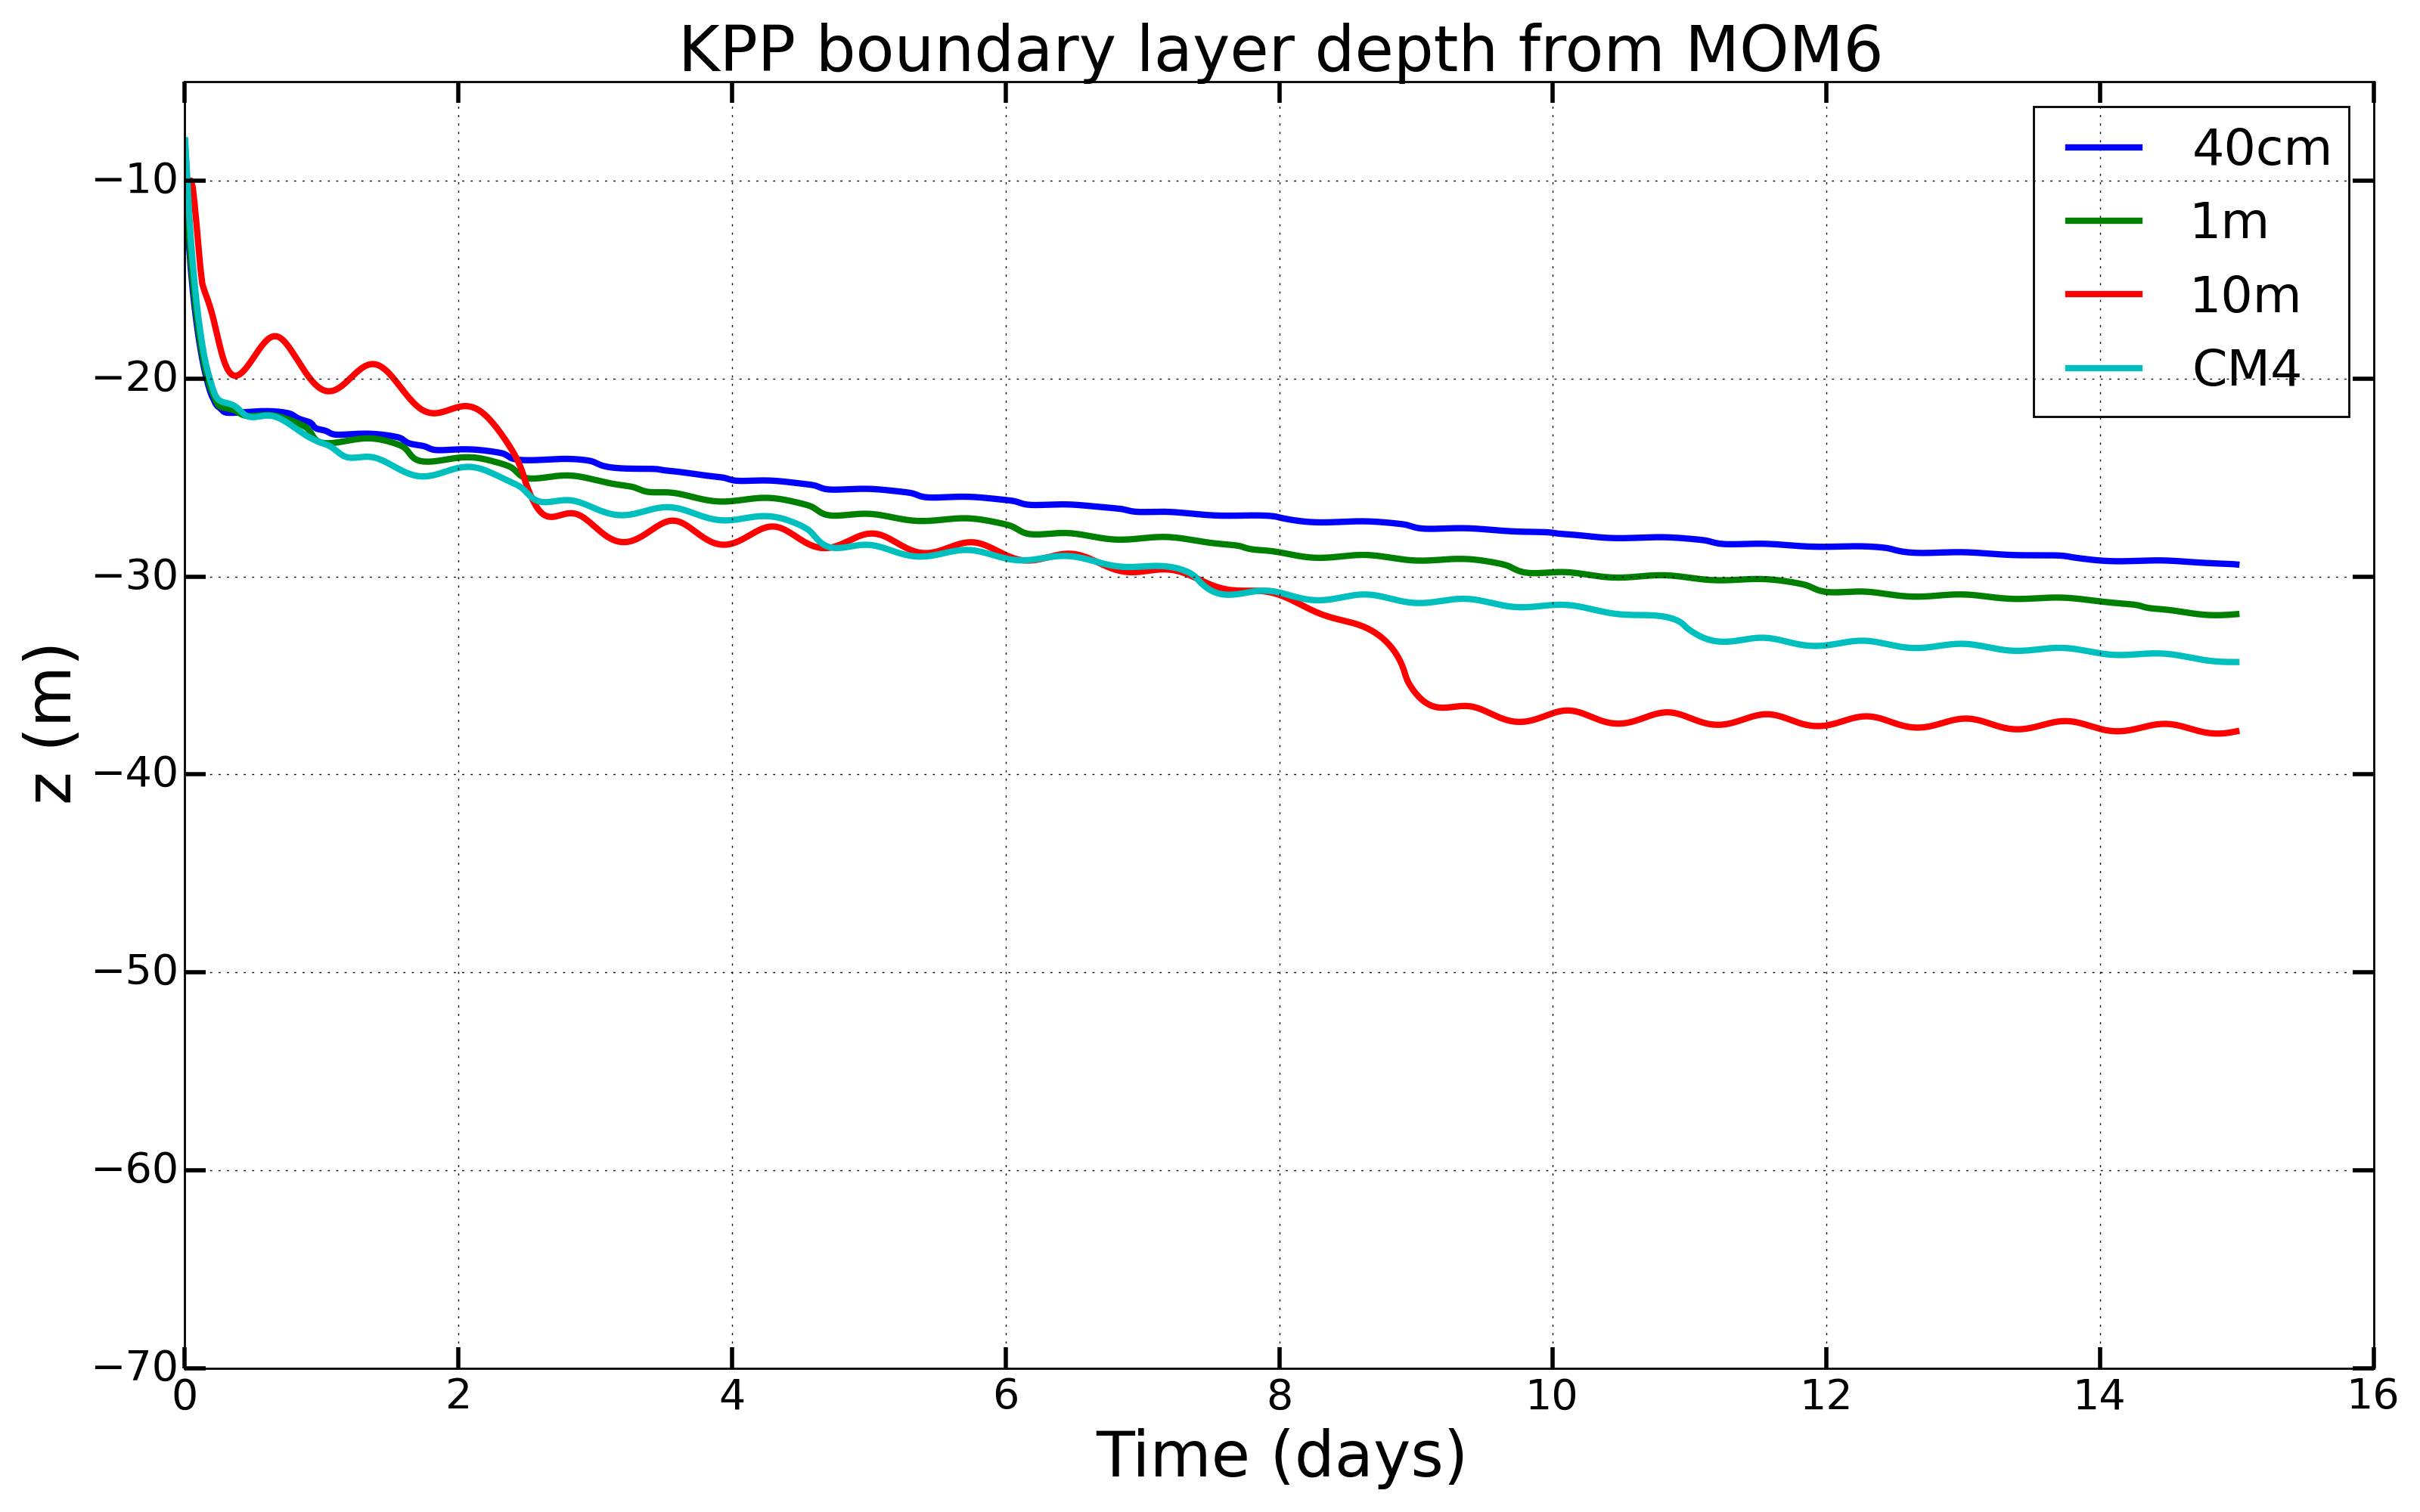
\includegraphics[angle=0,width=5cm]{./figs/MOM6/wind_only_KPP_MOM6_bldepth.png}
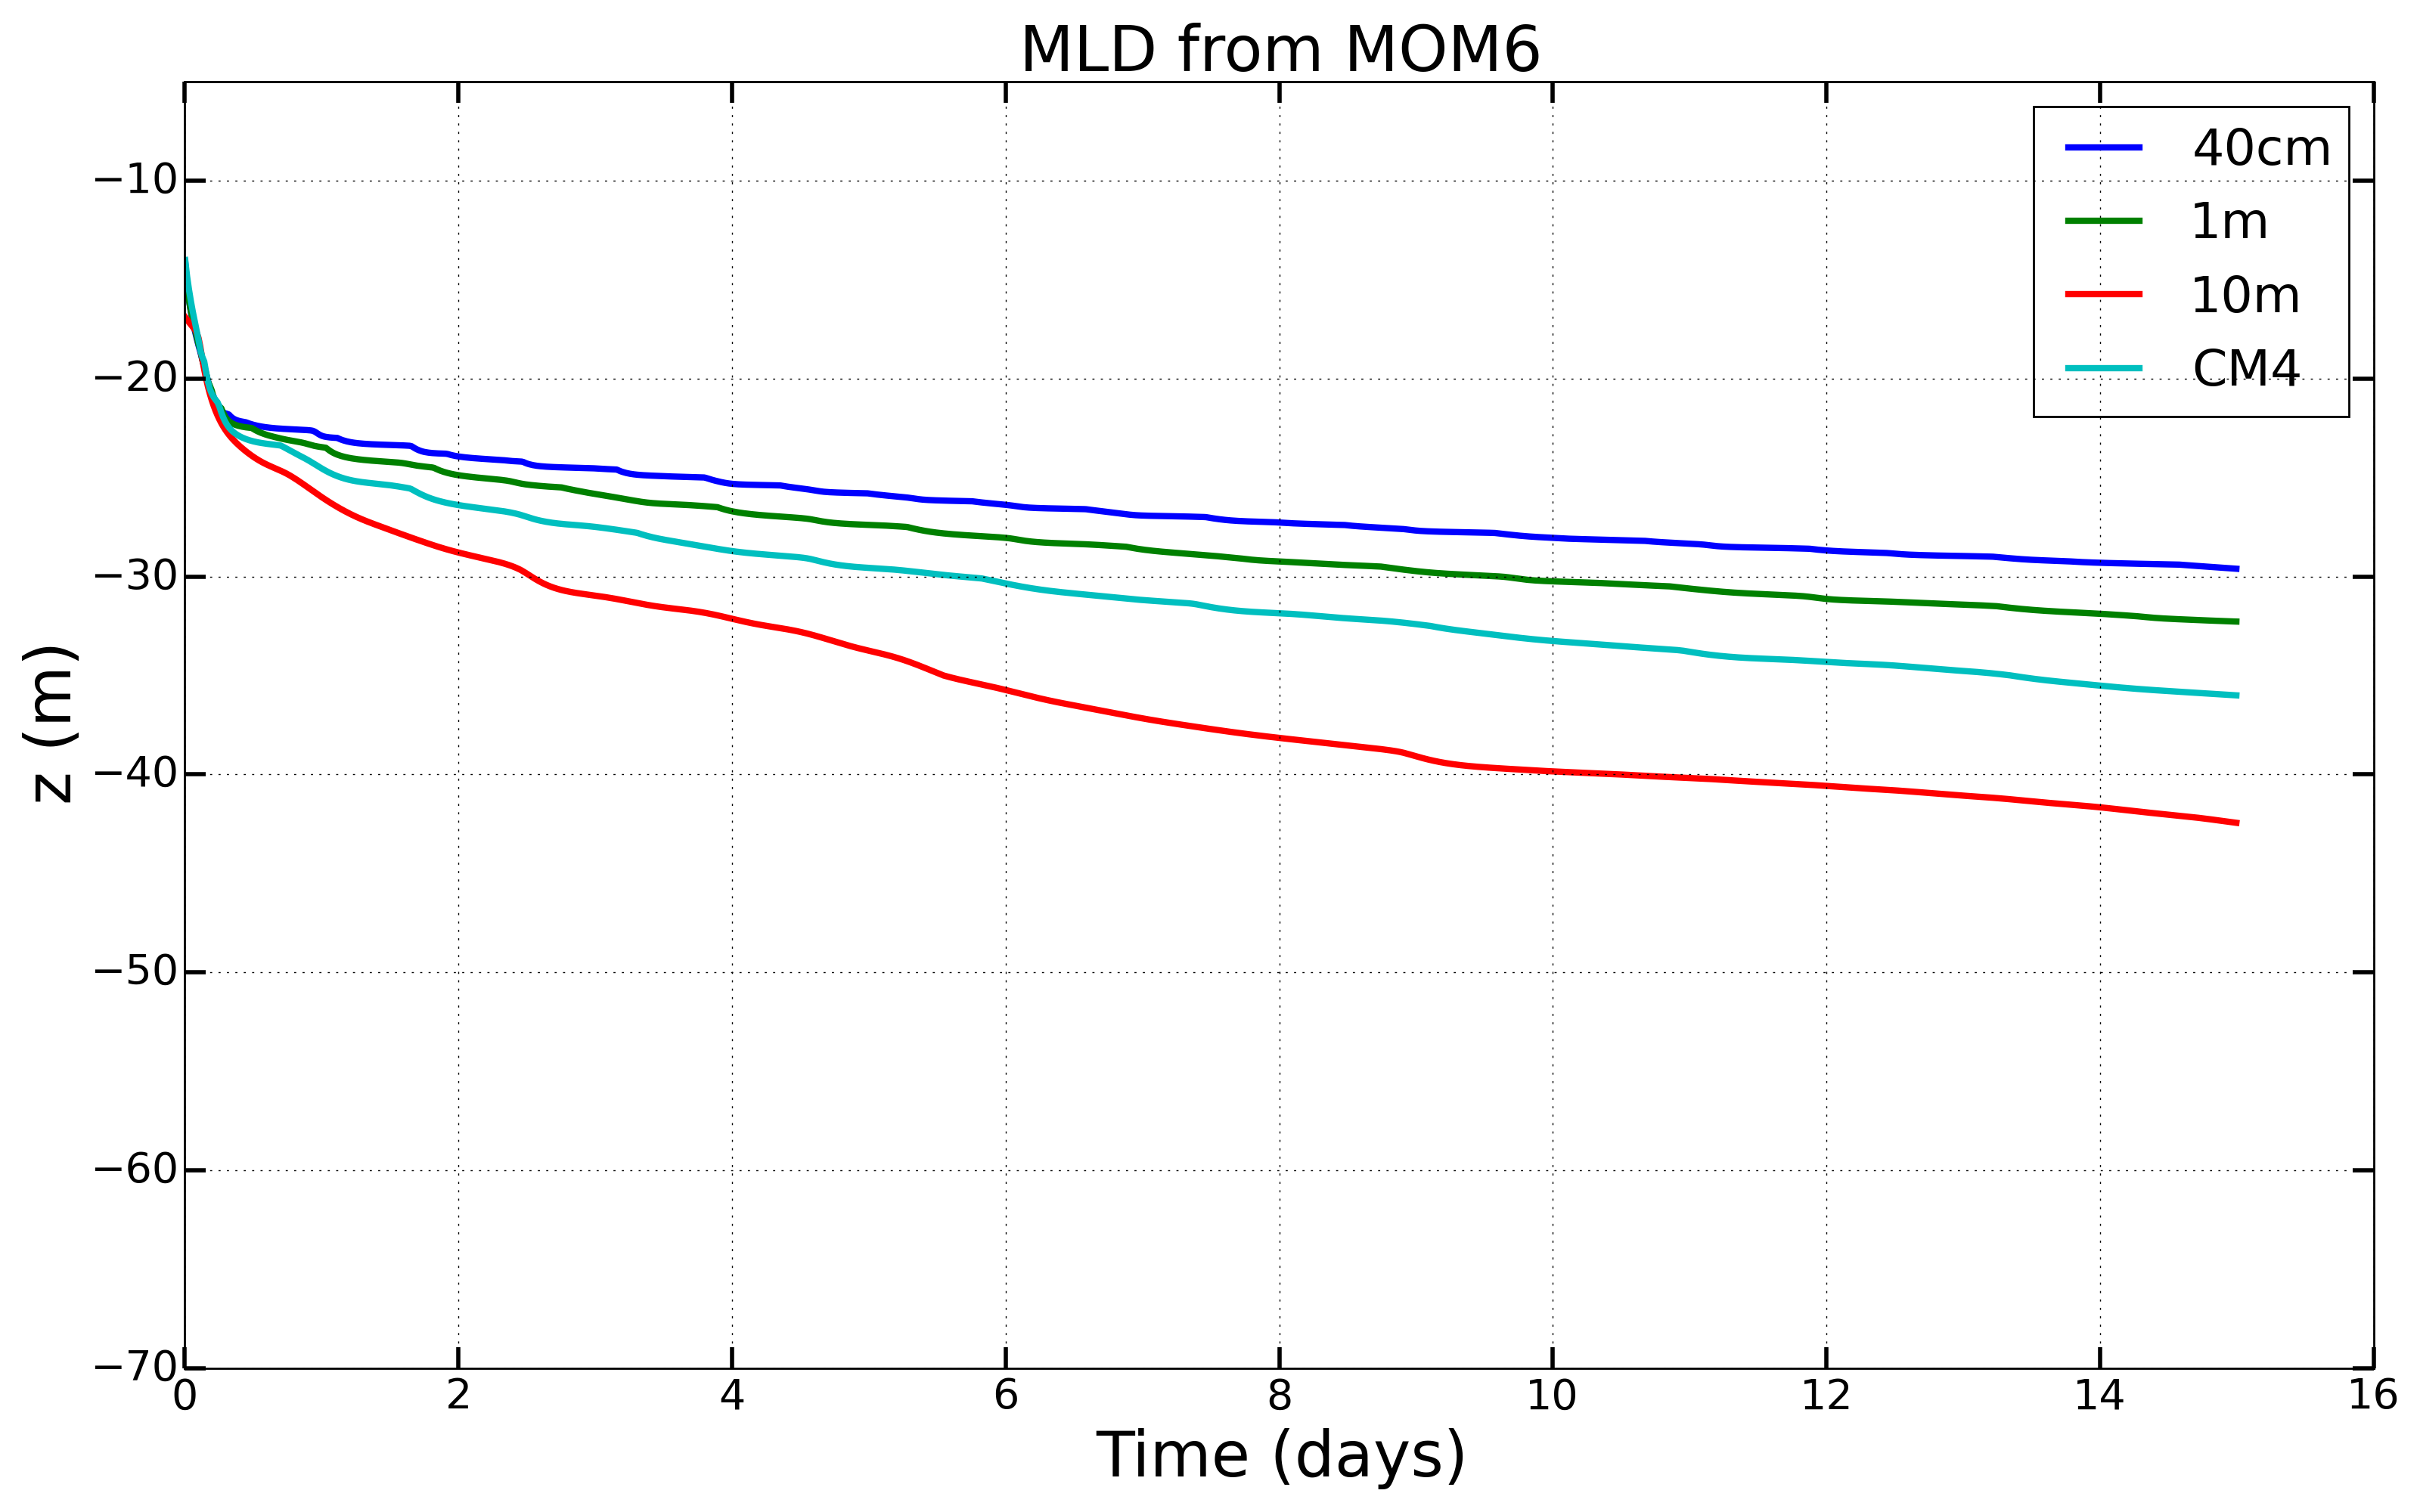
\includegraphics[angle=0,width=5cm]{./figs/MOM6/wind_only_KPP_MOM6_mld.png}
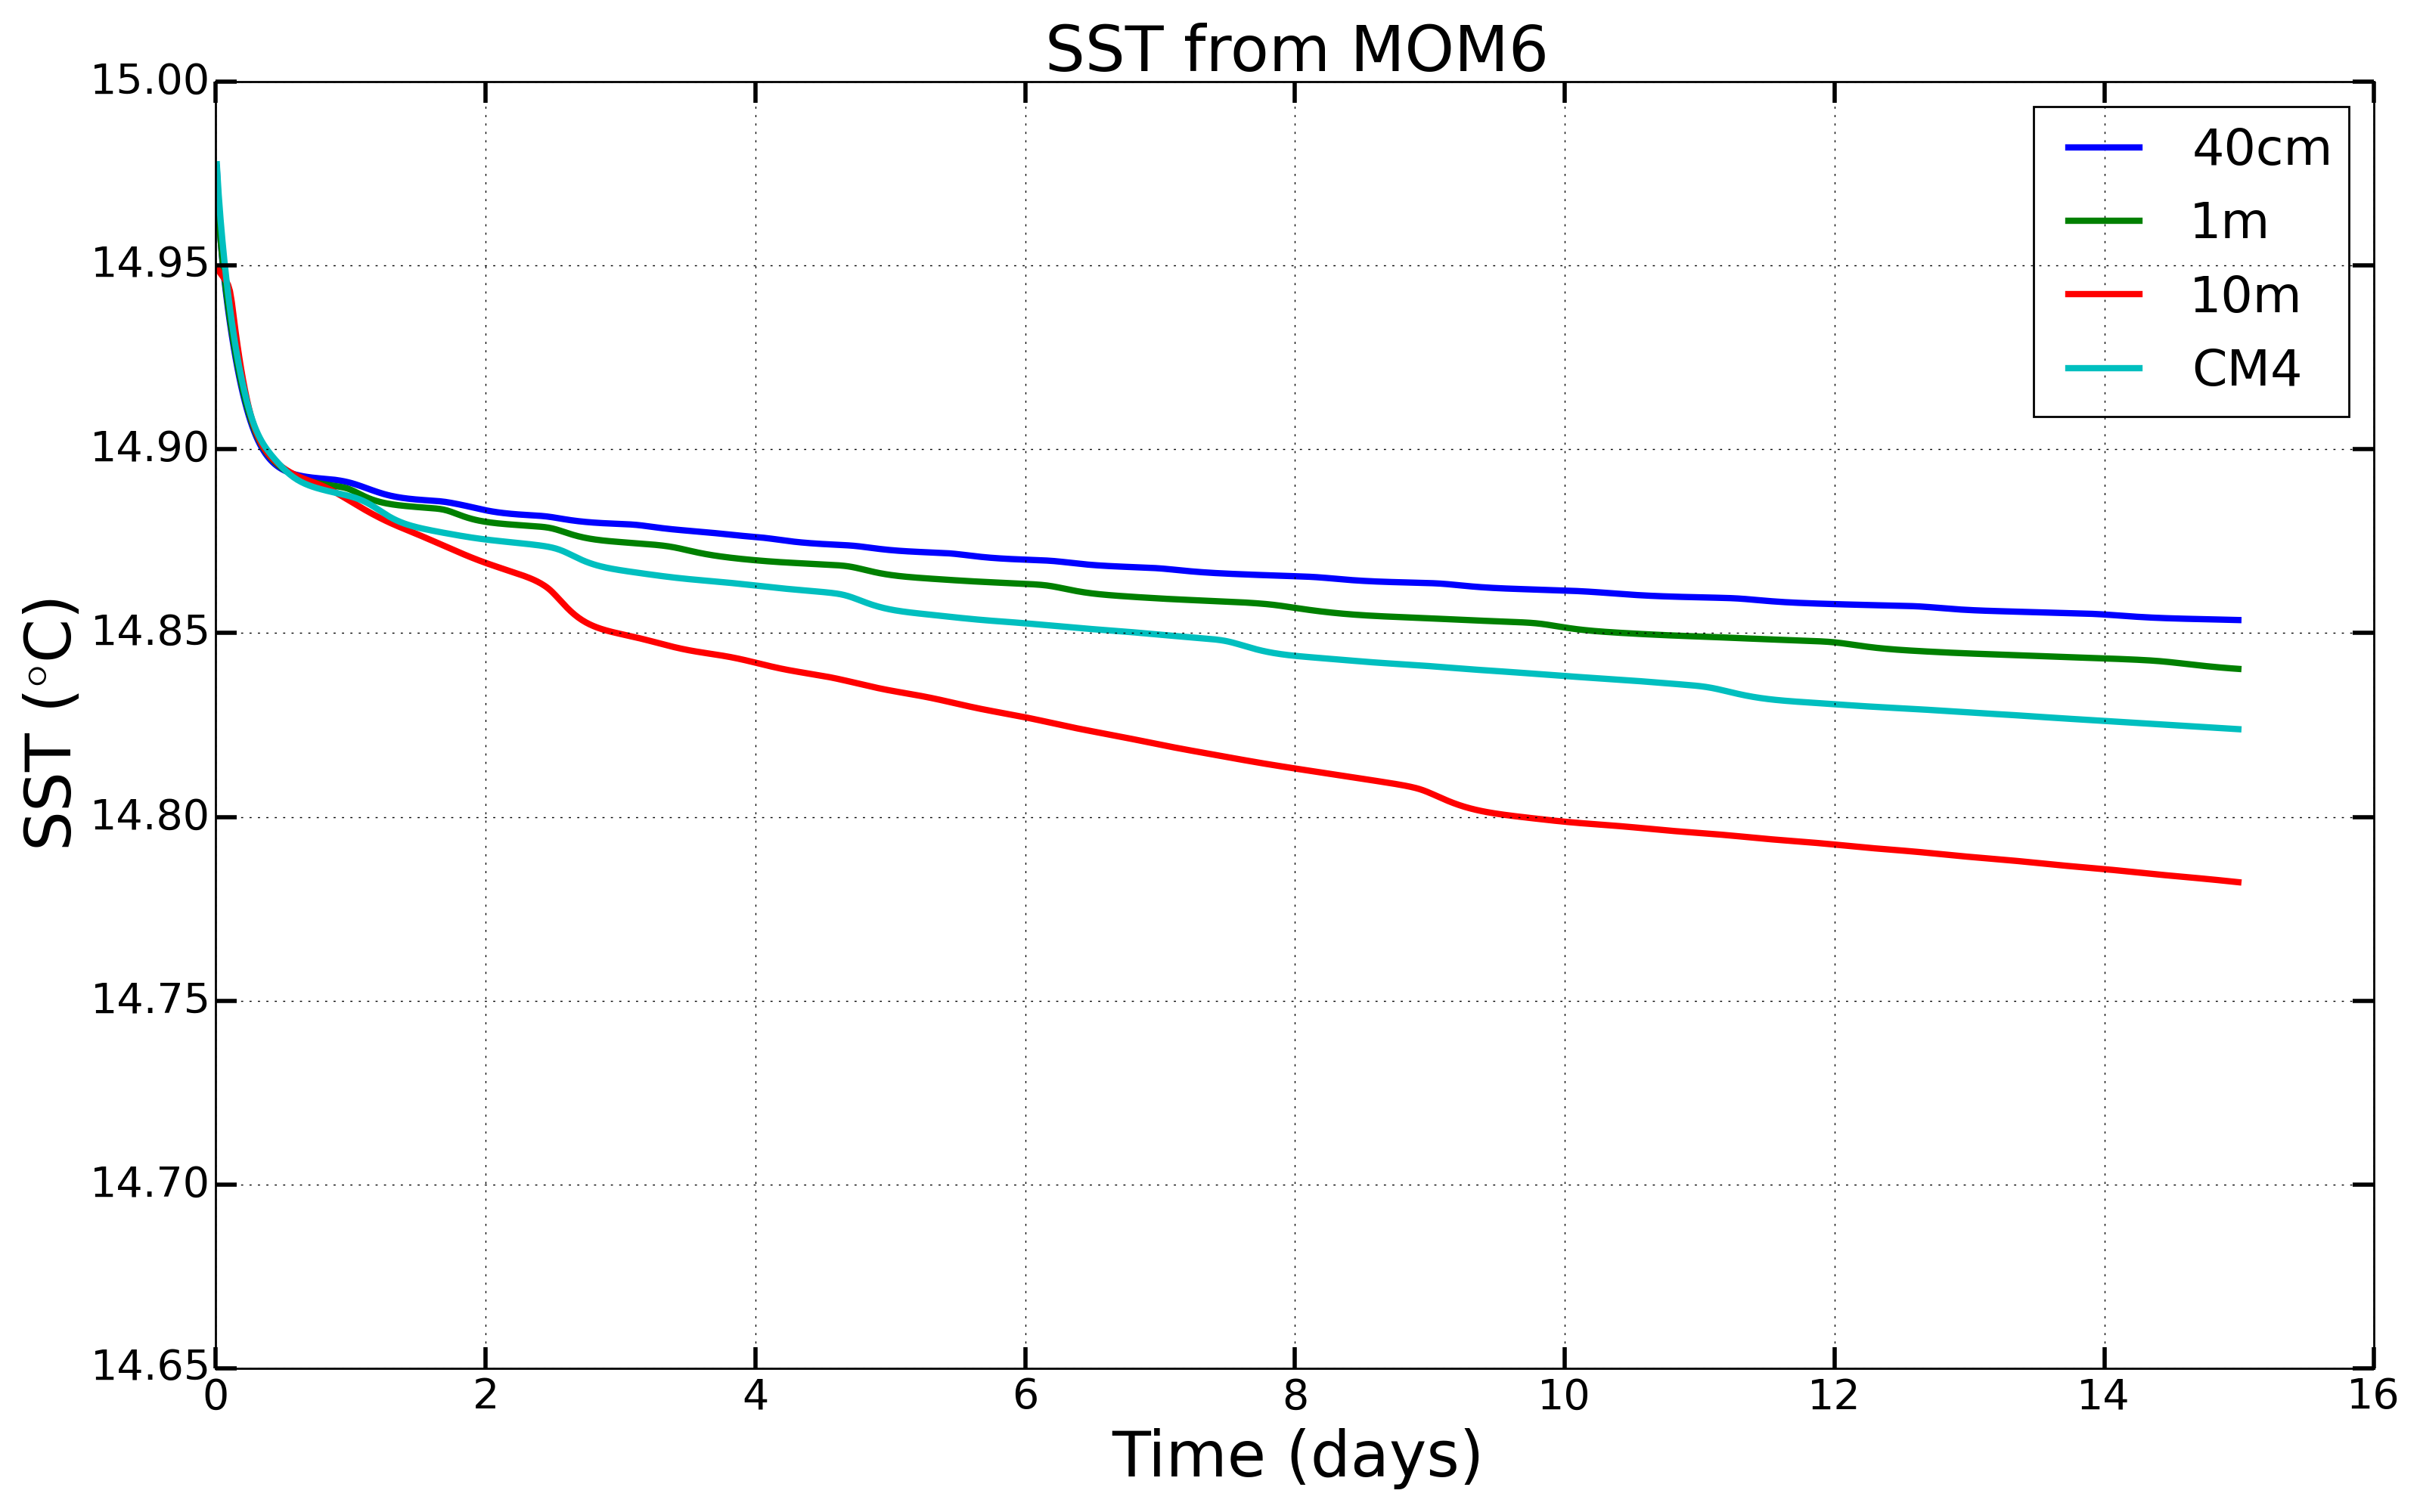
\includegraphics[angle=0,width=5cm]{./figs/MOM6/wind_only_KPP_MOM6_SST.png}
\caption[KPP BL depth, ML depth, and SST from MOM6 for
winds-alone]{\sf Time series for KPP boundary layer depth (left
  panel), mixed layer depth (middle panel), and SST (right panel) for
  the wind test case (constant zonal wind stress and zero surface
  buoyancy forcing) as realized in MOM6.  The mixed layer depth is
  diagnosed as the depth where density differs from the surface by
  $0.003~\mbox{kg}~\mbox{m}^{-3}.$}
\label{fig:MOM6_SST_bldepth-wind_alone}
\end{center}
%\rule{\textwidth}{0.005in}
\end{figure}
%%%%%%%%%%%%%%%%%%%%%%%%%%%%%%%%%%%%%%%%%%%%%%%%%%%%%%%%%%%%%%%%%%%%%%%%


%%%%%%%%%%%%%%%%%%%% %%%%%%%%%%%%%%%%%%%%%%%%%
\begin{figure}[h!t]
%\rule{\textwidth}{0.005in}
\begin{center}
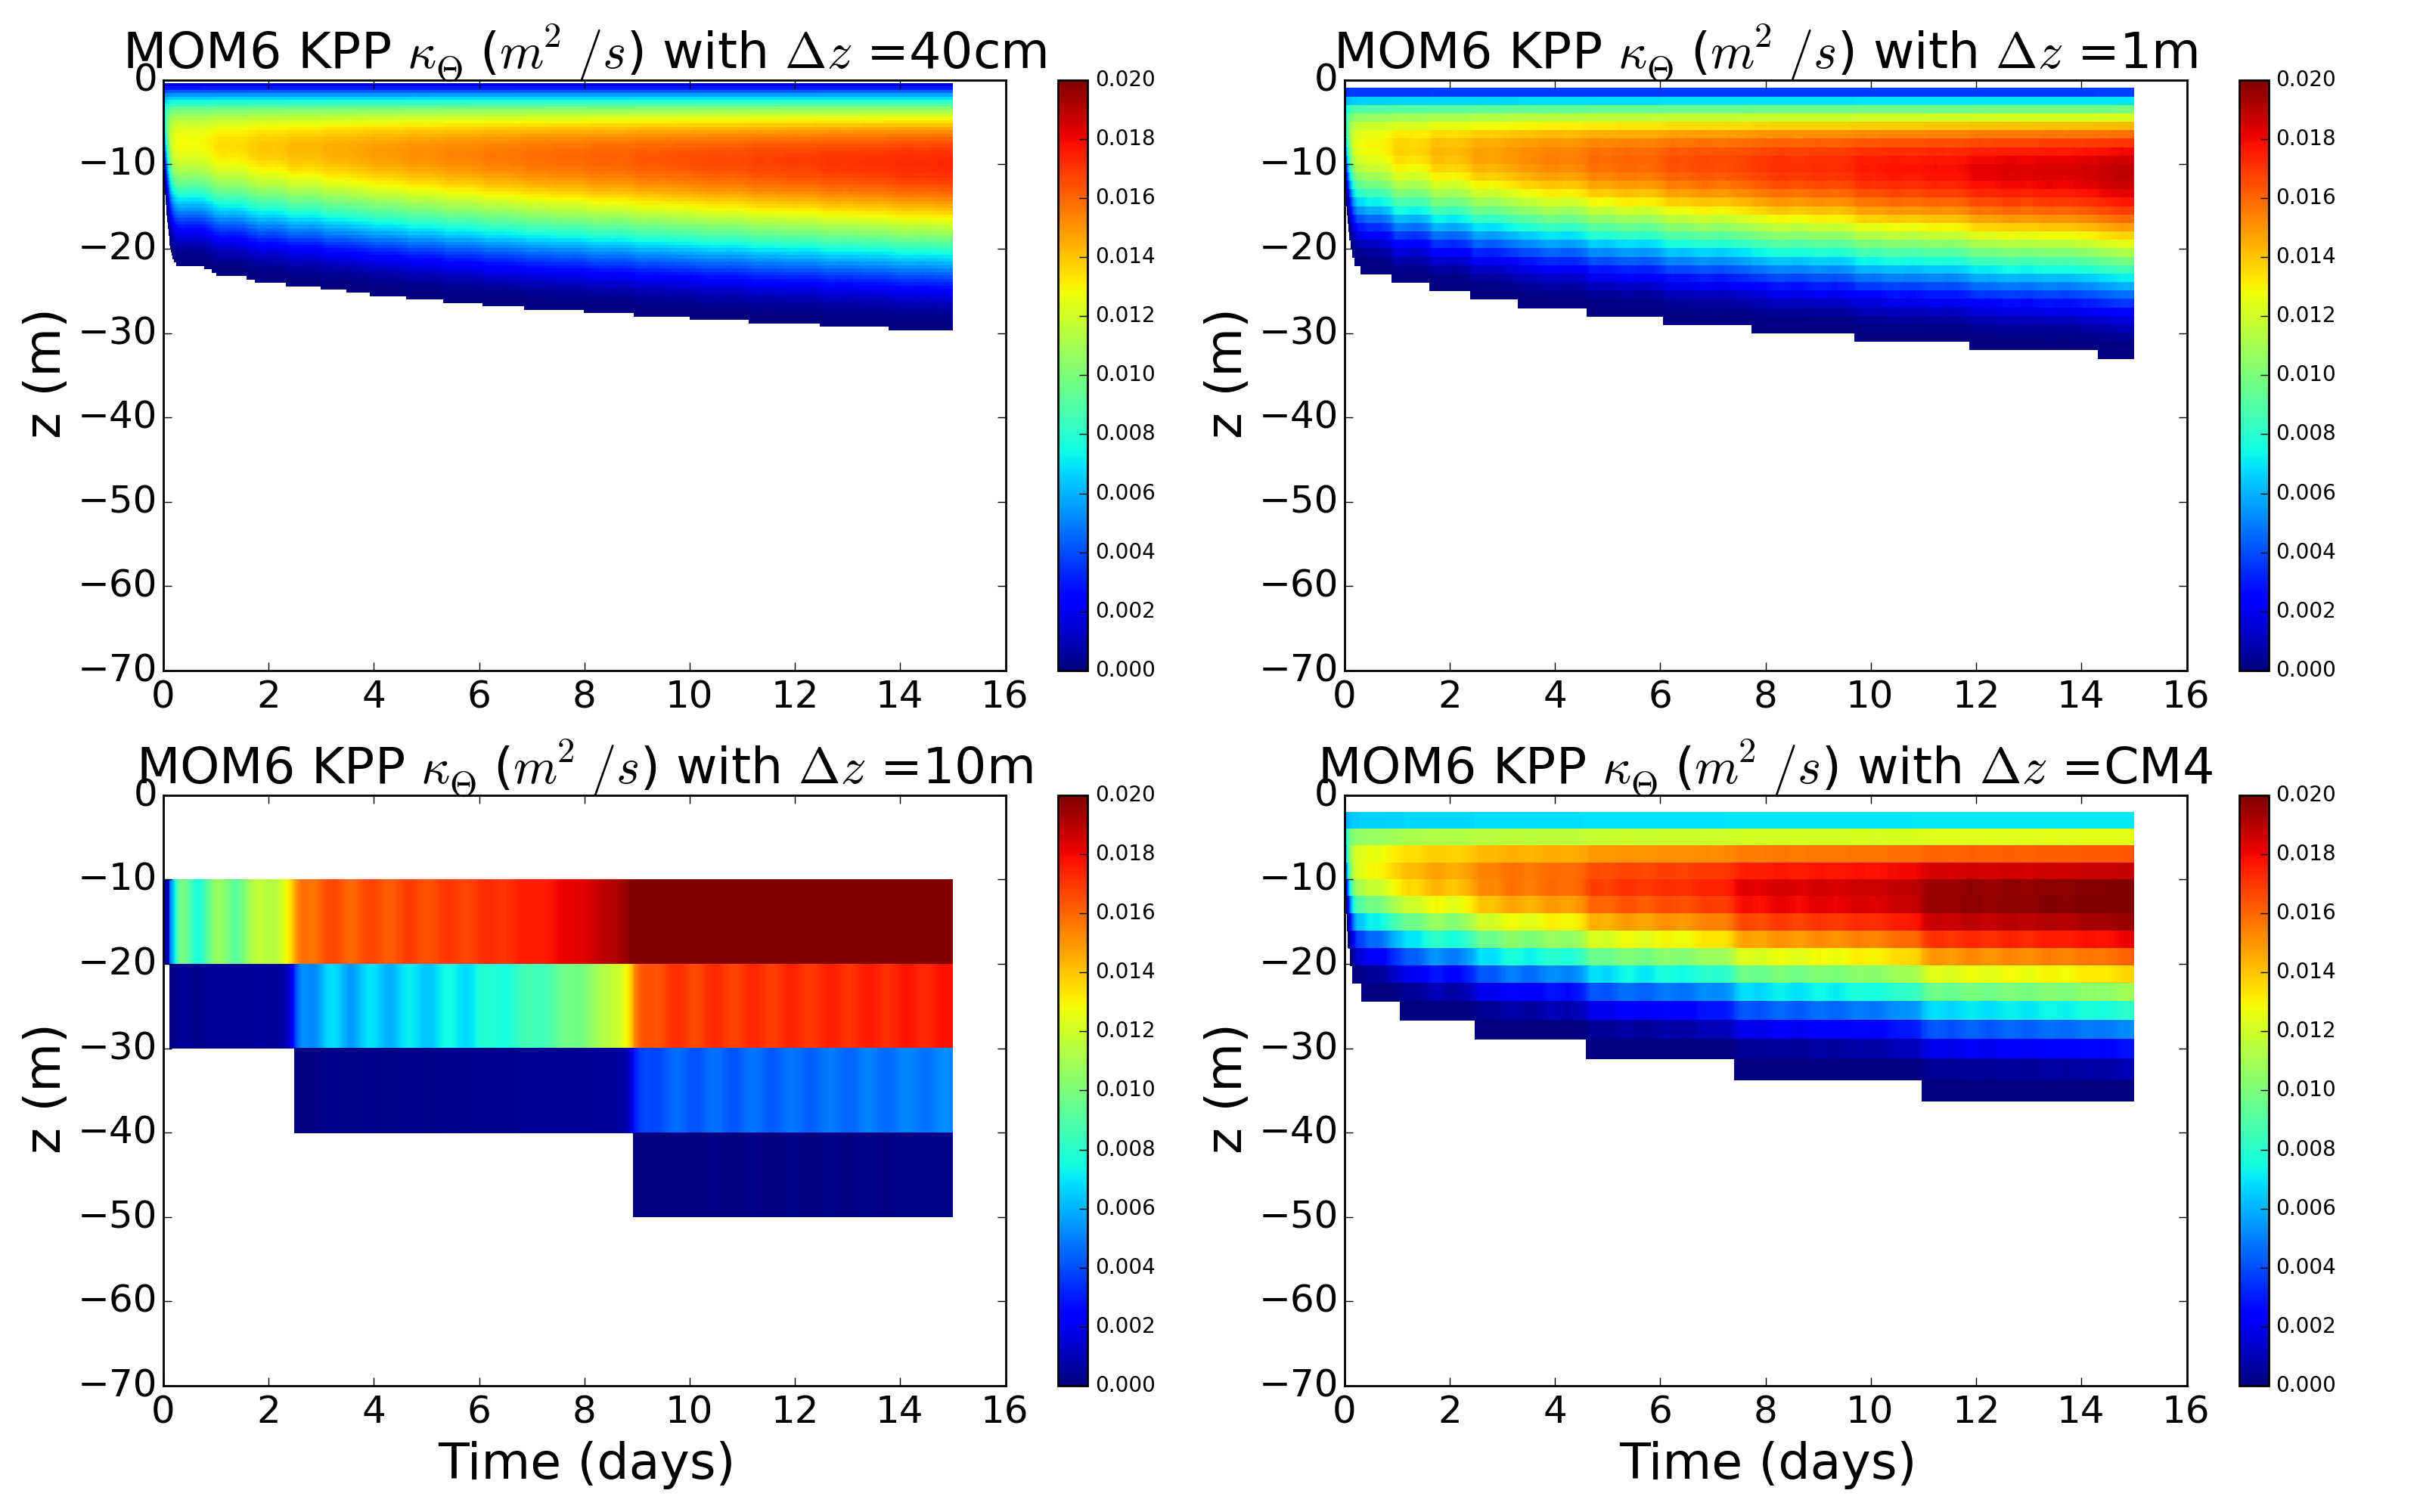
\includegraphics[angle=0,width=14cm]{./figs/MOM6/wind_only_KPP_MOM6_KPP_diffusivity.png}
\caption[KPP diffusivity from MOM6 for winds-alone test]{\sf Time
  series for the KPP vertical diffusivity for the wind test case
  (constant zonal wind stress and zero surface buoyancy forcing) as
  realized in MOM6 using four different vertical grid resolutions.
  The diffusivity is centered on the bottom interface of a grid cell,
  with the first nonzero value at the bottom of the surface cell.}
\label{fig:MOM6_KPP_diffusivity-wind_alone}
\end{center}
%\rule{\textwidth}{0.005in}
\end{figure}
%%%%%%%%%%%%%%%%%%%%%%%%%%%%%%%%%%%%%%%%%%%%%%%%%%%%%%%%%%%%%%%%%%%%%%%%


%%%%%%%%%%%%%%%%%%%% %%%%%%%%%%%%%%%%%%%%%%%%%
\begin{figure}[h!t]
%\rule{\textwidth}{0.005in}
\begin{center}
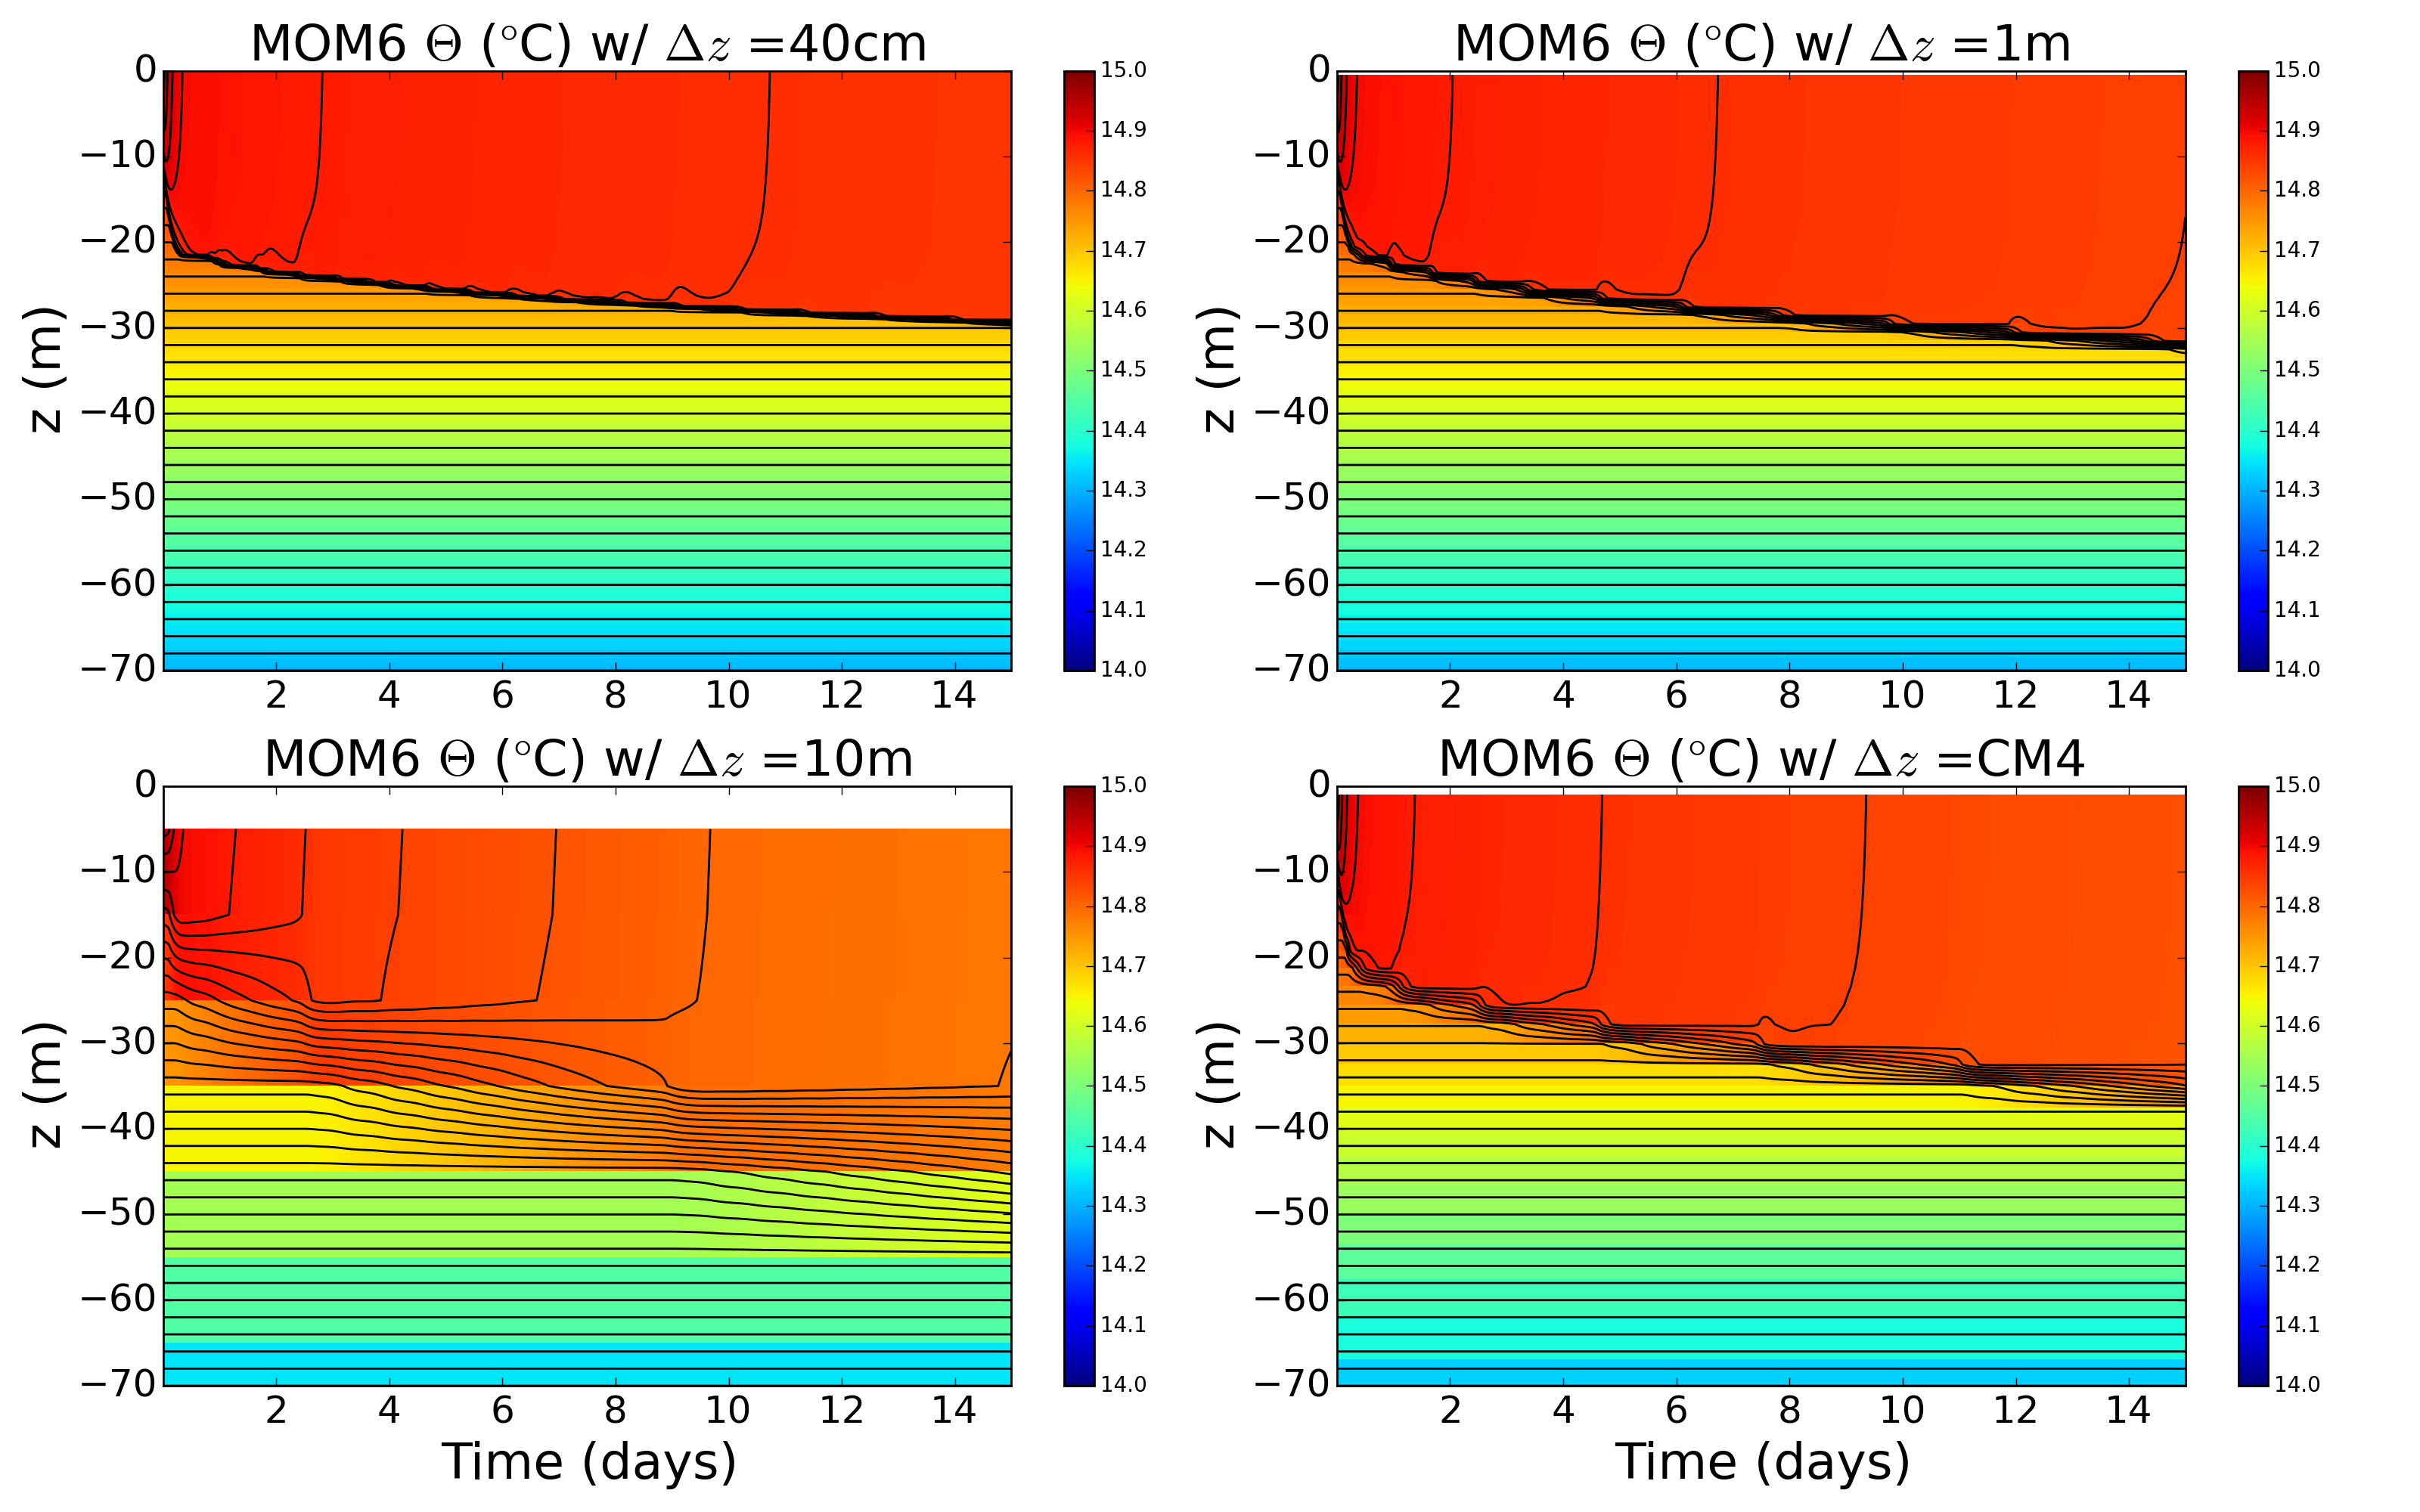
\includegraphics[angle=0,width=14cm]{./figs/MOM6/wind_only_KPP_MOM6_temp.png}
\caption[Temperature from MOM6 for winds-alone test]{\sf Time series
  for temperature in the wind test case (constant zonal wind stress
  and zero surface buoyancy forcing) as realized in MOM6 using four
  different vertical grid resolutions.  The temperature is located at
  the center of a grid cell, with the first nonzero value at the
  center of the surface cell.}
\label{fig:MOM6_temp-wind_alone}
\end{center}
%\rule{\textwidth}{0.005in}
\end{figure}
%%%%%%%%%%%%%%%%%%%%%%%%%%%%%%%%%%%%%%%%%%%%%%%%%%%%%%%%%%%%%%%%%%%%%%%%

%%%%%%%%%%%%%%%%%%%% %%%%%%%%%%%%%%%%%%%%%%%%%
\begin{figure}[h!t]
%\rule{\textwidth}{0.005in}
\begin{center}
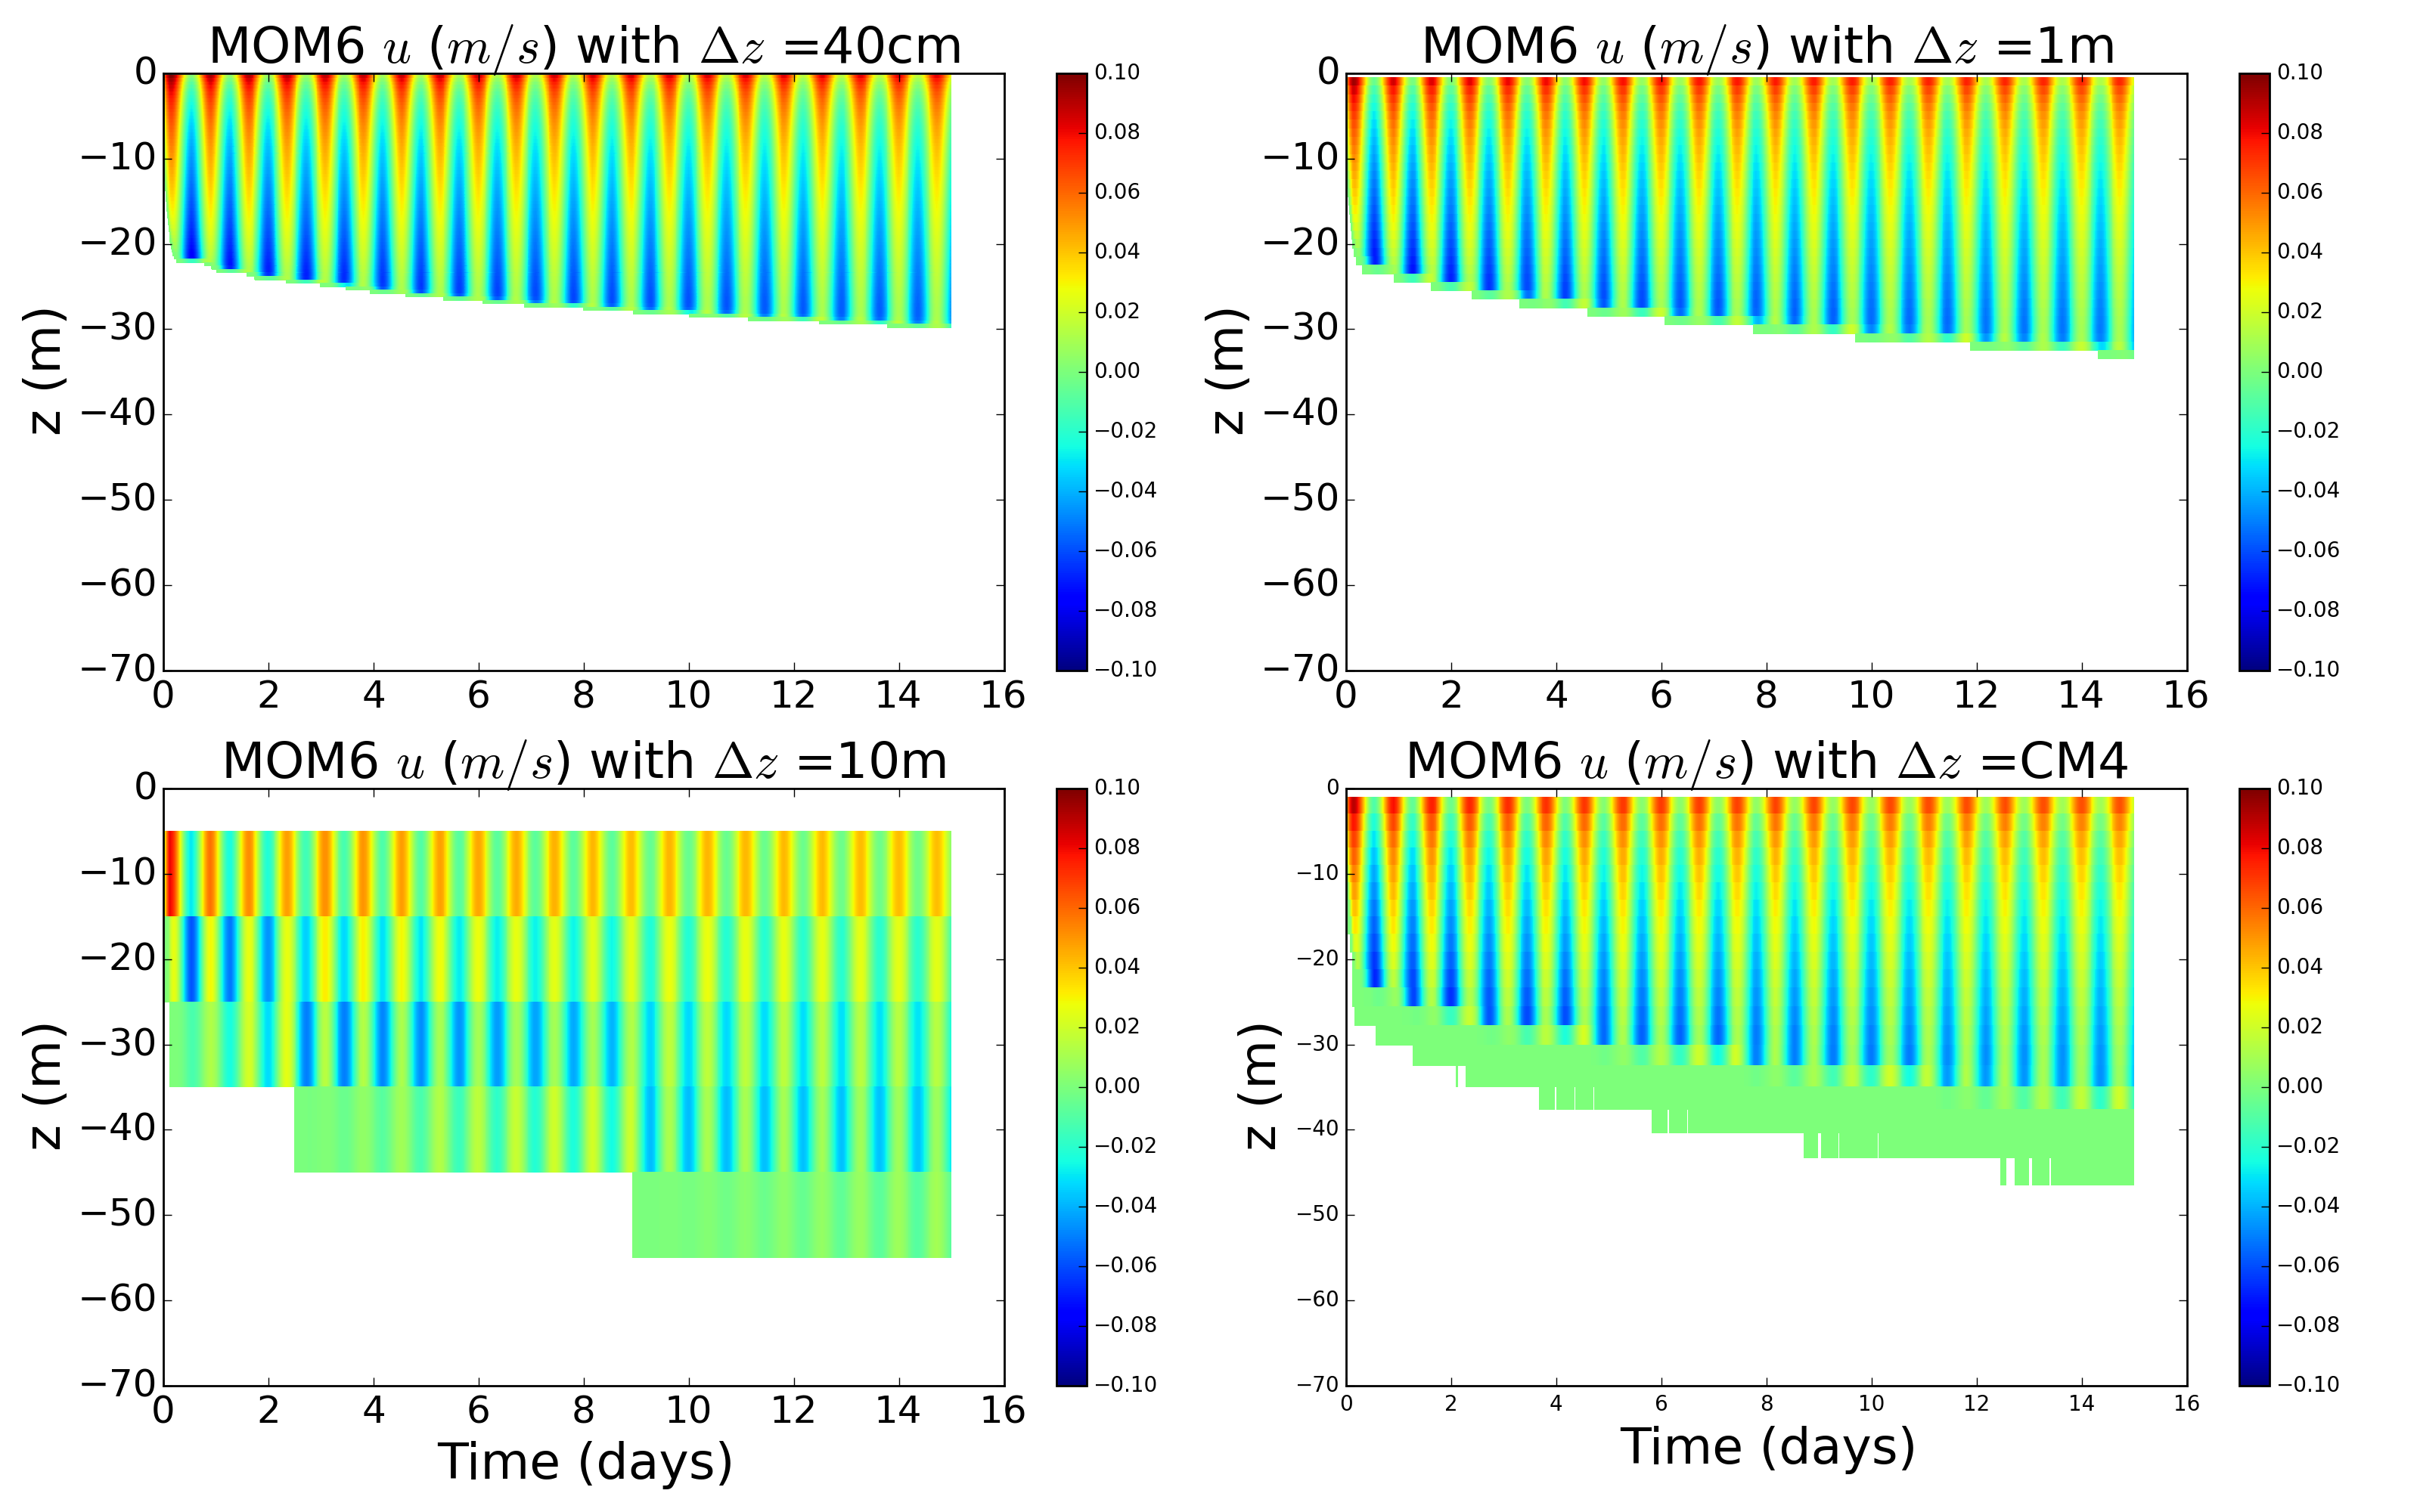
\includegraphics[angle=0,width=14cm]{./figs/MOM6/wind_only_KPP_MOM6_zonal_velocity.png}
\caption[Zonal velocity from MOM6 for winds-alone test]{\sf Time
  series for zonal velocity in the wind test case (constant zonal wind
  stress and zero surface buoyancy forcing) as realized in MOM6 using
  four different vertical grid resolutions. The velocity is centered
  on the center of a grid cell, with the first nonzero value at the
  center of the surface cell.}
\label{fig:MOM6_zonal-wind_alone}
\end{center}
%\rule{\textwidth}{0.005in}
\end{figure}
%%%%%%%%%%%%%%%%%%%%%%%%%%%%%%%%%%%%%%%%%%%%%%%%%%%%%%%%%%%%%%%%%%%%%%%%





